\chapter{The Ending of Image}

This chapter follows the sixth Brockwood Park dialogue in \emph{The Transformation of Man}, credited to J. Krishnamurti and preserved through the Krishnamurti Foundation Trust source material, with curation by LazyingArt LLC through Video2Book. There is no blackboard mathematics in the validated material, and no frame-backed equation or diagram survives for this lecture. The mathematical form used here is therefore deliberately schematic: equations and diagrams are not physics formulae but compact notation for the order of the inquiry. The point is to preserve the movement of the dialogue: from the large question of transformation, down into ordinary relationship, through image, hurt, pleasure, observer, time, and finally to the unresolved question of meditation.

\section{From Transformation To Ordinary Life}

The dialogue begins with an enormous question: what will change man? More precisely, what can bring about a radical transformation in the total consciousness of a human being? The question is first addressed to a scientist, but the scientific standing of the speaker is immediately set aside. Expertise may be useful in its own field, but it is not the authority here.

That refusal matters. It prevents the inquiry from becoming an appeal to theory. The question is not, ``What does science say about consciousness?'' It is, ``What, in the life one actually lives, can bring about change?'' Krishnamurti presses the point by speaking as the ordinary viewer: a person who goes to the office or the factory, who has a family, poverty, fatigue, conflict, and very little time. Such a person may listen to philosophical dialogue and say that it is too remote, too vague, too far away.

The first movement, then, is a descent from abstraction to contact. The question of transformation must be brought nearer. It must be tested where life is already burning.

\begin{equation}
\text{radical transformation}
\;\not\leftarrow\;
\text{scientific authority}
\end{equation}

This is not an anti-scientific statement. It is a boundary. The dialogue is not going to use knowledge, prestige, or expert procedure as the instrument of inward transformation. The problem has to be found in ordinary life itself.

\section{Relationship As The Field Of Inquiry}

Bohm proposes the first practical field: daily relationship. Krishnamurti accepts it immediately. Relationship is where the question touches the office, the factory, the golf course, the home, sex, children, insult, disappointment, hope, desire for success, and the movement of wanting more.

This is the chapter's first real reduction. We do not begin with consciousness as an abstraction. We begin with relationship, because relationship is where consciousness is exposed. The state of relationship reveals the state of the mind that enters it.

\begin{equation}
\text{daily life}
\;\longrightarrow\;
\text{relationship}
\;\longrightarrow\;
\text{image exposed}
\end{equation}

The question then becomes more exact: what is the source of my relationship? Why is it so often wounded, forced, demanding, disappointed? The answer that emerges is image. I have an image of myself, an image of you, and an image of how you should be in relation to me. When that image is not confirmed, there is disappointment, hurt, and conflict.

\subsection{Question \& Answer}

\paragraph{Question.}
Why begin with relationship rather than with a general doctrine of consciousness?

\paragraph{Answer.}
Because relationship is the concrete test. If consciousness is filled with images, this will not first appear as a theory; it will appear as demand, hurt, fear, dependence, comparison, and expectation in relationship. To begin with relationship is to begin where the image is already acting.

\section{Image As The Block In Relationship}

The dialogue now names the structure more sharply. A person may have an image of security, an image of pleasure, an image of entitlement, an image of what is just, an image of what a wife or husband should do, an image of how another person should complete one's own feeling of oneself. These images do not simply sit in the mind. They organize action.

A compact model is useful, as long as we remember that it is a note-taking aid, not a formal equation:

\begin{equation}
\text{self-image}
+
\text{image of the other}
+
\text{claim}
\;\longrightarrow\;
\text{forced relationship}
\;\longrightarrow\;
\text{conflict}.
\end{equation}

The decisive phrase in the dialogue is that any form of image about another or about oneself prevents the beauty of relationship. The point is not that one should adopt a better image. A better image would still be an image. Nor is the point that relationship should obey an ideal. The ideal itself would become a new image through which the other person is judged.

The image is not passive representation. It is an active demand for confirmation. It says: you should be this way, because that would complete my picture. It says: I am secure only if you behave like that. It says: I am hurt because the picture I had of myself has been struck. In this sense, the image does not merely distort relationship; it replaces relationship with a model of relationship.

\begin{figure}
\centering
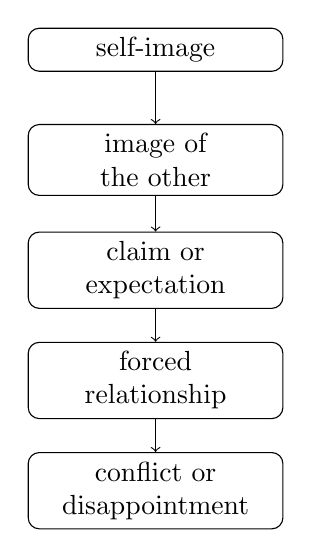
\begin{tikzpicture}[x=1cm,y=1cm]
\node[draw, rounded corners, text width=3.0cm, align=center] (a) at (0,0) {self-image};
\node[draw, rounded corners, text width=3.0cm, align=center] (b) at (0,-1.4) {image of\\the other};
\node[draw, rounded corners, text width=3.0cm, align=center] (c) at (0,-2.8) {claim or\\expectation};
\node[draw, rounded corners, text width=3.0cm, align=center] (d) at (0,-4.2) {forced\\relationship};
\node[draw, rounded corners, text width=3.0cm, align=center] (e) at (0,-5.6) {conflict or\\disappointment};

\draw[->] (a) -- (b);
\draw[->] (b) -- (c);
\draw[->] (c) -- (d);
\draw[->] (d) -- (e);
\end{tikzpicture}
\caption{A transcript-backed reconstruction of relationship under image. The diagram is editorial, not copied from a board.}
\end{figure}

\section{Energy, Seriousness, And The Refusal To Delegate}

The dialogue then asks whether one has the energy to watch the image in all the places where relationship occurs. Energy here is explicitly not scientific energy. It means vitality, seriousness, drive, the available intensity of attention.

At first the examples are obvious: drink, smoke, useless chatter, moving from pub to pub. But the deeper movement is not moral condemnation. These are named as wastage when the importance of relationship has actually been seen. If relationship is of the greatest importance, then whatever dulls the mind or confirms despair becomes visible as waste.

The argument can be written as a conditional rule:

\begin{equation}
\text{seeing the importance of relationship}
\;\longrightarrow\;
\text{seeing what wastes energy}.
\end{equation}

The dialogue immediately goes deeper. One of the most subtle images is the image that someone else will do it for me, or that I cannot do it myself. That image may then confirm itself: despair leads to escape, escape proves incapacity, incapacity demands rescue. The loop sustains the very image it complains of.

\begin{align}
\text{I cannot do it myself}
&\longrightarrow \text{escape or dependence} \\
&\longrightarrow \text{confirmation of incapacity} \\
&\longrightarrow \text{renewed demand that another act for me}.
\end{align}

This is why the dialogue introduces responsibility. Not responsibility as self-improvement rhetoric, but as the fact that nobody can transform my relationship for me. If another person lives beautifully, I may admire or imitate, but imitation leaves my relationship as it was. The inquiry therefore returns to the one who is listening.

Krishnamurti then widens the point: you are the world, and the world is you. The phrase is not a slogan. It means that the structure of suffering, anxiety, confusion, fear, hope, deception, and conditioning is not merely private. It is found across cultures and lives. The individual problem is not isolated from the human problem.

\section{Consciousness As Interrelated Images}

Once relationship has been shown to be structured by image, the dialogue gathers the examples into a larger claim: consciousness as we know it is filled with images. These images are not separate fragments. They are interrelated, and they are centered on the self-image.

\begin{equation}
\text{consciousness as known}
\approx
\{\text{interrelated images centered on the self}\}.
\end{equation}

The symbol here is only a notation of convenience. The dialogue is not defining consciousness in a technical system. It is noticing that the content of ordinary consciousness is occupied by images: what I am, what I was, what I should become, what you did to me, what I deserve, what I fear, what I hope to get.

This makes the demand much more radical. To have no image is not merely to improve one relationship. It means that consciousness as one knows it is called into question. It is not a request to polish the self-image; it is the ending of image-making.

At this point a natural question appears: how am I to do it? The dialogue refuses the question in that form. The ``how'' implies a method; the method implies a self who will apply it; that self is already the image-maker.

\subsection{Question \& Answer}

\paragraph{Question.}
Why does asking ``how do I end image-making?'' recreate the image-maker?

\paragraph{Answer.}
Because the question quietly puts the ``me'' back at the center. The method may sound impersonal, but it implies someone who will practice, achieve, compare, and arrive. That someone is not outside the image-process. It is one of its central forms.

\begin{align}
\text{how shall I do it?}
&\longrightarrow \text{method} \\
&\longrightarrow \text{me applying the method} \\
&\longrightarrow \text{the image-maker restored}.
\end{align}

The refusal of method is therefore not laziness or vagueness. It is a precision. If the problem is the image-making self, then a method centered on that self carries the problem forward under a new name.

\section{Pleasure, Hurt, And Registration}

The dialogue next slows down into a concrete example. My wife calls me an idiot. The event is registered in the brain. Thought takes it over; memory enters; the image I have about myself is hurt. The same structure applies to flattery. If I am praised, the image swells; thought elaborates it; pleasure appears. Hurt and pleasure are then described as two sides of the same coin.

The process may be written as a small update rule:

\begin{equation}
\text{event}
\;\longrightarrow\;
\text{registration}
\;\longrightarrow\;
\text{thought/memory}
\;\longrightarrow\;
\text{image}
\;\longrightarrow\;
\text{hurt or pleasure}.
\end{equation}

\paragraph{Worked example.}
Take the insulting sentence, ``You are an idiot.'' The dialogue's sequence is not that pure perception simply receives sound. The event is registered, and then thought and memory take it over. The old image of oneself, perhaps as competent, respectable, or deserving recognition, is struck. The result is hurt.

\begin{enumerate}
\item A phrase is heard: insult.
\item The brain registers the event.
\item Thought and memory take possession of the registration.
\item The self-image is activated.
\item The image, with insult as its content, is hurt.
\end{enumerate}

For flattery the content changes, but the machinery does not.

\begin{table}
\centering
\begin{tabular}{|p{0.35\linewidth}|p{0.35\linewidth}|}
\hline
\textbf{Flattery} & \textbf{Insult} \\
\hline
Registered by the brain & Registered by the brain \\
\hline
Thought and memory take it over & Thought and memory take it over \\
\hline
Image expands as pleasure & Image contracts as hurt \\
\hline
The self-image is reinforced & The self-image is wounded \\
\hline
\end{tabular}
\caption{A compact comparison of the same image-process under two different contents.}
\end{table}

The dialogue's sharper notation is:

\begin{equation}
\text{flattery} \longrightarrow \text{image-as-pleasure},
\qquad
\text{insult} \longrightarrow \text{image-as-hurt}.
\end{equation}

And then, more generally,

\begin{equation}
\text{pleasure} \sim \text{hurt},
\end{equation}

where the symbol means only that they are two sides of the same image-process. It does not mean that pleasure and hurt feel the same. It means that both are sustained by image, registration, thought, and memory.

The next obstacle is whether old hurts and future hurts must be handled separately. The dialogue says no. The remembered hurt and the anticipated hurt work by the same principle. A present insult may awaken the past; a remembered insult may act like a fresh one. Therefore the inquiry does not divide the hurts by date. It looks at the structure of image itself.

\begin{equation}
\text{past hurt}
\;\not\perp\;
\text{future hurt}.
\end{equation}

Again, the notation is only shorthand: past and future hurt are not separate principles. They are movements of the same image.

\section{The Observer Is The Observed}

The central question now appears: how am I to look at the image? The difficulty is immediate. If I look with another image, then the observer is already part of the problem. I may look with the image that I must suppress the image. I may look with the image that right relationship will give me a beautiful life. I may look with the image that I am serious, intelligent, or capable. The question becomes: is the observer different from that which he observes?

The first answer is the ordinary assumption: yes. Tradition, language, and habit all say that there is an observer here, and an image there. But the dialogue asks us to examine that division. If the observer is different from the observed, then there is an interval. In that interval time enters, and with time come adjustment, escape, substitution, and conflict.

\begin{equation}
\text{observer} \neq \text{observed}
\;\longrightarrow\;
\text{interval}
\;\longrightarrow\;
\text{time}
\;\longrightarrow\;
\text{conflict}.
\end{equation}

Bohm then brings in a careful distinction about reality. Some reality is sustained by thought. Some reality, such as nature, is independent of thought. The self, however, is ordinarily felt to be a reality independent of thought, as though there were a real observer who possesses thoughts and looks at images. The dialogue questions this.

The observer is reconstructed as past: memories, experiences, accumulated incidents, old movements of becoming, and projections into the future. The ``me'' that appears to look at the past is itself made of the past.

\begin{equation}
\text{past memories}
\;\longrightarrow\;
\text{me as image}
\;\longrightarrow\;
\text{projected future}.
\end{equation}

This is psychological time. It is not clock time. It is the movement by which the image of myself at three, five, ten, seventeen, and now is strung together as though a substantial observer had traveled through a developmental sequence. The dialogue asks whether that movement is an actuality or an image. The answer is not obtained by intellectual agreement. It must be seen directly.

The conjuring-trick analogy helps. Before the trick is seen through, one appears to perceive a woman being cut in half. After the trick is seen, one does not perceive the same event more accurately; one sees that the previous perception was organized by missing something essential. Likewise, as long as the observer is assumed to be separate, the image has power. When the observer is seen as part of the image-process, the problem changes.

\begin{equation}
\text{observer} = \text{observed}.
\end{equation}

This identity is not algebra. It is the dialogue's central insight in compact form. The observer is the past, the movement of thought, the maker of image. If that observer is not separate, then the image-maker has no independent standing.

\begin{figure}
\centering
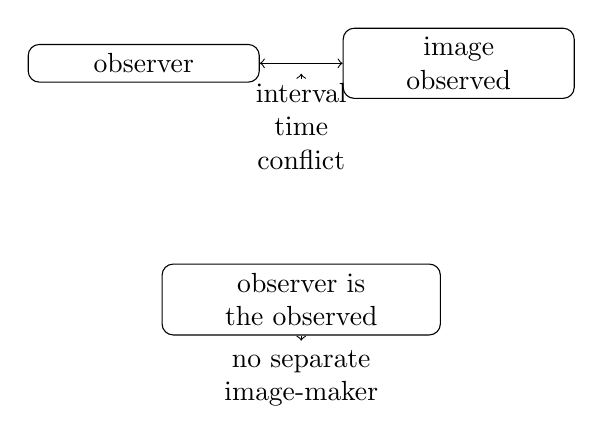
\begin{tikzpicture}[x=1cm,y=1cm]
\node[draw, rounded corners, text width=2.7cm, align=center] (o1) at (-2.0,0) {observer};
\node[draw, rounded corners, text width=2.7cm, align=center] (i1) at (2.0,0) {image\\observed};
\node[text width=3.0cm, align=center] (t1) at (0,-0.8) {interval\\time\\conflict};
\draw[<->] (o1) -- (i1);
\draw[->] (0,-0.2) -- (t1);

\node[draw, rounded corners, text width=3.3cm, align=center] (o2) at (0,-3.0) {observer is\\the observed};
\node[text width=3.5cm, align=center] (n2) at (0,-4.0) {no separate\\image-maker};
\draw[->] (o2) -- (n2);
\end{tikzpicture}
\caption{A two-stage reconstruction of the observer division: first separation, then the seeing that the observer is not apart from the image.}
\end{figure}

\subsection{Question \& Answer}

\paragraph{Question.}
Is the observer different from the image being observed?

\paragraph{Answer.}
The dialogue says no. The observer appears different because thought presents the self as though it were an independent reality looking at its own contents. But the observer is made of memory, past experience, preference, fear, and image. Therefore the observer is not outside the observed image. The observer is the observed.

The same point is then turned around:

\begin{equation}
\text{no thinker apart from thought},
\qquad
\text{no image-maker apart from image}.
\end{equation}

If there is no observer in the old sense, the command ``look at the image'' changes meaning. It is no longer a divided act in which one fragment controls another. It is the direct seeing of the image-process without a separate center claiming authority over it.

\section{When Image-Making Ends}

After the observer and observed have been brought together, a residual objection appears: what about hidden images? Are there deep, underground images that must be unearthed one by one? The dialogue treats this very carefully. It does not build a theory of the unconscious. It says that within this inquiry, once the observer is seen as the observed, the one who would dig, expose, analyze, and possess hidden content is no longer standing outside the field.

The local formulation is strong:

\begin{equation}
\text{observer} = \text{observed}
\;\longrightarrow\;
\text{no separate image-maker}
\;\longrightarrow\;
\text{image-making ends}.
\end{equation}

This must not be turned into a general psychological doctrine. It is the dialogue's consequence within its own logic. If the observer is the maker of images, and if that observer is no longer separate, then the image-process no longer has the same center.

The discussion then opens into meditation. Krishnamurti asks what happens when there is no movement of thought as image-making. Time, in the psychological sense, is the movement of thought from the past into projection. If that movement ends, what remains? The dialogue does not answer with a technique. It does not prescribe Zen, Hindu meditation, guru practice, or any system. It says that all such activity, if carried on within the same consciousness of fear, anxiety, image, and image-maker, remains inside the same area.

\begin{equation}
\text{thought as image-making ends}
\;\Longrightarrow\;
\text{consciousness as known is transformed}.
\end{equation}

But the arrow is not a theorem. It is the edge of the inquiry. Thought still has its right place in knowledge and practical functioning. What ends is thought as the maker of self, image, fear, pursuit of pleasure, anxiety, division, and turmoil.

\subsection{Question \& Answer}

\paragraph{Question.}
Is this the death of the self, and what does the lecture leave open?

\paragraph{Answer.}
The dialogue calls it the death of the self, but immediately resists reducing that phrase to destruction. It is the ending of the image-making center. What remains is not presented as an experience, because experience would again imply an experiencer. The lecture stops with the question: when thought as psychological time ends, what takes place?

\section{Summary}

The lecture's progression is exact. It begins with the question of radical transformation and refuses the authority of expertise. It brings the question down to the ordinary viewer. It selects relationship as the field where the problem is visible. It shows that relationship is distorted by images of oneself, others, entitlement, security, pleasure, and hurt. It treats energy as seriousness, not as a scientific quantity. It exposes the dependency-image that someone else will do the work.

From there the inquiry becomes structural. Consciousness as we know it is largely interrelated images centered on the self. Asking for a method restores the self as image-maker. Insult and flattery show the machinery of registration, thought, memory, image, hurt, and pleasure. Past and future hurt are not separate principles. Finally, the observer who tries to look at the image is seen to be part of the image-process itself.

The closing question is deliberately left open. If the observer is the observed, if the thinker is not apart from thought, and if the image-maker has no separate existence, then what happens when thought as image-making time ends? The lecture does not package the answer. It leaves the reader at the threshold where meditation, transformation, and the ending of image become one serious question.